
\chapter{The ``software crisis'' and encapsulation}

This book is going to dive deeply into a huge pile of nuts and bolts. But
before we take the leap into particulars, it's important to stand briefly at
the precipice and understand why we're jumping. What does ``object-oriented''
mean? What problem was it intended to solve? When was it invented and why?

\section{Ancient history}

A long time ago, in our own galaxy, a situation emerged which has been labeled
\textbf{the software crisis}. This crisis didn't happen at an instant in time;
it was a set of disagreeable circumstances which gradually evolved until it
became unbearable. The crisis is usually dated somewhere in the 1970's. This
was just as the high-tech computing industry was really starting to heat up,
on its way to permanently changing the lives of almost everyone on the planet.

Now ``crisis'' is an alarming word, designed to get your attention. It's worth
asking what all the hubbub was about. The immediate symptom may not strike you
as a three-alarm fire: it was simply that software projects were tending to
overrun their schedules.

The '70's were not a very plug-and-play era, since standards had not yet
evolved to facilitate intercompatibilities between devices or programs. So the
focus was often on building complete systems from the ground up. Engineering
teams would plan releases of key product lines that involved numerous
components, such as system architecture, hardware design and integration, data
collection and organization, system and network configuration, and software
development at both the operating system and the end user levels.

What managers discovered was that consistently, the \textit{software}
components of projects were coming in late and over-budget. Sometimes, they
didn't get finished at all. When they did, they were buggy and brittle. And
they were especially vulnerable to requirements changes: if circumstances were
discovered during the project that required a change in the way the software
needed to work, the software team was often strikingly unable to adapt to
this. They could be set back weeks or months to implement even a modest
change.

This astonished everyone at the time. After all, ``\textit{soft}ware'' -- a
pun on ``hardware'' -- was a term intended to convey the flexible, malleable
nature of computer programs as contrasted with physical devices. Software was
supposed to be easy to write and easy to change. That was the point. You
didn't need complex manufacturing processes: you needed a desktop computer and
a text editor. And you (seemingly) didn't face challenges of scale the way you
did with hardware: you could run out of room to put logic circuits on a chip
or a motherboard, but there was no limit to the size of a text file. 

So building complex stuff quickly, and turning on a dime when necessary, ought
to be easy to do in software. Right?

\subsection{Quantifying the crisis}

I've never seen any hard data quantifying the budget overruns and delays that
software projects faced in the 1970's. It's possible to sketch it
conceptually, though. Take a look at Figure~\ref{fig:complexityCurve}. This is
my attempt to show the main dynamic at work.

\begin{figure}[ht]
\centering
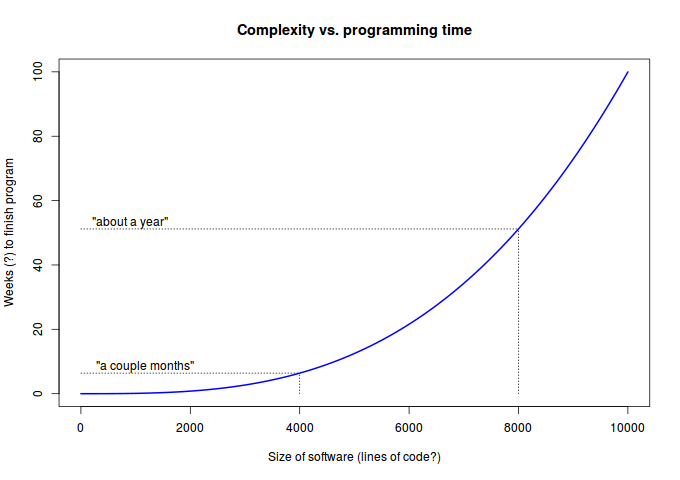
\includegraphics[width=0.9\textwidth]{complexityCurve.png}
\caption{The software crisis quantified: how long it took to complete a
program of various sizes. (Conceptual.)}
\label{fig:complexityCurve}
\end{figure}

On the $x$-axis is some measure of the \textit{complexity} of a proposed
computer program. Now complexity is devilishly difficult to quantify --
\textit{League of Legends} is more complex than \textit{Angry Birds}, but by
how much? Twice as complex? Ten times? A hundred times? I'll have a better
answer to that in a few paragraphs, but for now, as a proxy we'll just use the
\textit{size} of the program, measured in \textbf{lines of code}\footnote{I
know what you're thinking, and you're right. Not all lines of code are equally
complex. Some of them are just variable assignments, whereas others are parts
of complicated loops or function calls. Heck, some are just comments. Heck,
some are actually \textit{blank}. While all true, this analysis is conceptual
anyway, and we can surely say that raw program length is at least
\textit{somewhat} related to complexity -- show me a real-life ten-line
program that's actually more complex than a real-life ten-thousand-line
program and I'll concede.\\By the way, ``lines of code'' is sometimes
abbreviated ``LOC.'' Even more common is the abbreviation ``KLOC'' for
``thousands of lines of code.''}.

On the $y$-axis is the corresponding amount of time it would take a
programming team of a certain size to design, build (code), and test the
program.\footnote{Note carefully that this has nothing to do with how long the
code takes to \textit{run}. We're talking about programmer-time here, not
CPU-time.} As with the $x$-axis, we're making all kinds of simplifying
assumptions here: we're not worrying about exactly how many developers
there are, how much experience they each have, what language they're writing
in, \textit{etc.} That's okay. The point of this exercise is simply to
recognize the nature of the curve, showing how these two fuzzy variables were
related in the '70's.

A daunting curve it is, too. And very counterintuitive to project managers.
One would assume that if a 4,000-line program took the development team a
couple of months to release, an 8,000-line program would take about twice that
long. After all, it's twice as many lines, right?

The reality was not even close. A program with twice as many lines could
easily take \textit{four} times as long to build...or six, or ten, or twenty.
Worse, the programs that were built were also very hard to \textit{change}.
Take a large enough program and try to add a feature, fix a bug, or support a
new data format, and you inevitably broke something else while making the
change. Then you fixed what you broke, but \textit{d'oh!!} broke something
else by doing so, \textit{etc.}

It was miserable, especially because advances in other areas (like hardware)
were making exciting technologies possible for the first time. Everyone was
rarin' to go, yet unexpectedly the software (supposedly the easy part) was
gumming up the works.

For a time, it almost seemed as if the human race had uncovered some built-in
limitation of the universe, like the speed of light. This hypothetical limit
might have been called ``maximum complexity,'' meaning the greatest amount of
sophistication one could build in to a single logical creation. That curve in
Figure~\ref{fig:complexityCurve} starts to go up fast. Maybe, people
depressingly thought, a functioning 200,000-line program isn't even
\textit{possible} to create? That threatened to put a damper on a lot of
expectations.

\section{Software and complexity}

Let's consider a different way to measure a program's complexity than simply
counting the lines of code. Instead, let's quantify its number of
\textit{dependencies}.

A \textbf{dependency} between two chunks of software (be they individual lines
of code, constructs like loops or if/else chains, functions, or something even
bigger) means that \textit{if one of them changes, the other may possibly be
affected.}

For instance, suppose I define a function \texttt{compute\_sales\_tax()} to
take one argument: the price of an item. It will return the sales tax on that
item as a simple percentage. We'll call that ``code chunk A.'' Now suppose
that I call the function in ``code chunk B'' as follows:

\begin{Verbatim}[fontsize=\small,samepage=true,frame=single]
   // In code chunk B...
   double item_price = 24.99;
   double total_price = item_price + compute_sales_tax(item_price);
\end{Verbatim}

We say that code chunk B has a dependency on A. If we were to change A to
require a second parameter (perhaps the state the customer lives in, since
different states have different laws about whether and how to collect sales
tax), that's great and all, \textit{but B immediately breaks}.

This example is a syntactic dependency: the compiler will fail when trying to
compile code chunk B because its parameter list is wrong (\textit{i.e.},
doesn't match A's). In general, though, dependencies are much broader than
just syntactic dependencies. They are also \textit{logical} dependencies, in
which one chunk of code depends on another's functionality working a certain
way.

For example, suppose that we change \texttt{compute\_sales\_tax()} in a
different way: instead of returning the sales tax, we make it return the cost
of the item \textit{plus} the sales tax. If our tax rate is 5\%, then the
original version of \texttt{compute\_sales\_tax(24.99)} would return 1.25 (the
sales tax on the item), but our new version would return 26.24 (the item's
price with its sales tax added in).

This may seem like a good change, since it prevents code like that in chunk B
from having to add the item's price back in. However, if we don't change B in
tandem with A, \textit{B breaks again}. It's not a compilation error this
time, but a logic error: B's \texttt{total\_price} variable is now going to
contain 51.23 because we didn't keep the two chunks of code in sync.

\subsection{Dependencies == complexity}

Now why do I bring all this up? Because it turns out that the \textit{length}
of a program was not the cause of the software crisis. Instead, it was
\textit{the number of dependencies} programs had. That turns out to be a
different, and more salient, measure of a program's complexity.

\begin{figure}[ht]
\centering
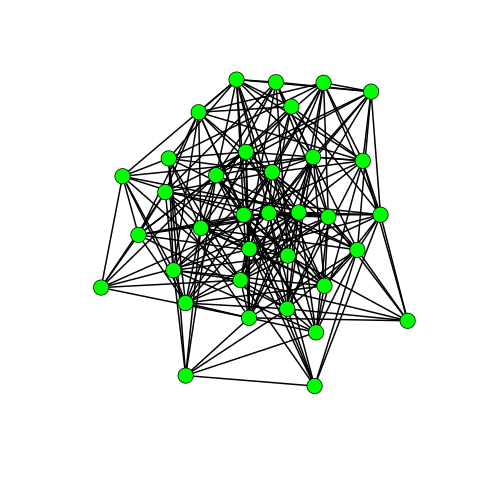
\includegraphics[width=0.45\textwidth]{highDependencies.png}
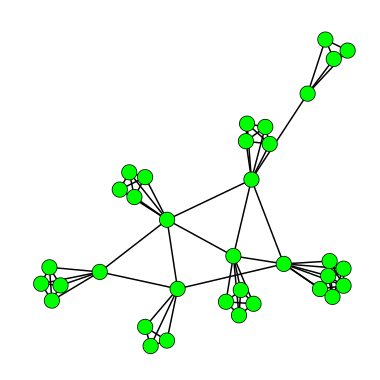
\includegraphics[width=0.45\textwidth]{lowDependencies.png}
\caption{Two programs, each with 35 code chunks. On the left, there are 230
dependencies. On the right, there are only 83.}
\label{fig:dependencies}
\end{figure}

Consider the two graphs\footnote{A \textbf{graph} in Computer Science terms is
a data structure that consists of \textbf{vertices} (or \textbf{nodes}) and
\textbf{edges} (or \textbf{links}) connecting them. They're often drawn with
circles and lines, as Figure~\ref{fig:dependencies} does.} in
Figure~\ref{fig:dependencies}. Imagine that each green circle represents one
chunk of code. Each line between circles represents a dependency: the two
chunks of code it connects rely on each other \textit{not} to change, because
if one of them changes, the other one might break.

The kind of program illustrated by the left-hand graph sometimes goes by the
name \textbf{spaghetti code}. You can see why just by looking at it.
Essentially, every line of code potentially depends on everything else.

By contrast, the right-hand graph depicts a \textbf{modular} program. It has
the same amount of functionality -- 35 green circles in each case -- but far
fewer dependencies between them (only about a third as many). Looking further,
you can see how most of the circles are ``hiding'' behind a gatekeeper circle
that connects to the main group. These circles are shielded from the morass of
dependencies by living in an isolated world, and only communicating with the
rest of the program through their gatekeeper.

Now look back at the left-hand graph. Choose one of the circles at random, and
imagine that it represents a chunk of code you need to change (maybe there's a
bug in it you have to fix, or you need to extend it in some way). Think about
the repercussions of that task. Fixing the green circle is a job in itself,
but once you've done so, how can you be sure you didn't break something else?
There might be twenty other chunks of code that depend on the first one
staying the way it was in order to work correctly. Just identifying all of
them is an enormous task, to say nothing of verifying that they all still
work, and fixing the ones that don't. And oh, by the way: if you \textit{do}
end up having to fix another green circle because your first change caused a
ripple effect...that second change is going to cause the exact same problem.

The situation is obviously much easier with the right-hand program. Again,
choose a circle at random, and then ask yourself how onerous it is to change
it. If you choose one of the many circles that are ``hiding'' behind their
gatekeeper, the possible damage is minuscule: only three or four other circles
might be affected. If you have to change a gatekeeper, the news is worse, but
still far better than it was with the left-hand program. Just count how many
dependencies there are for even the most densely connected circle of the
modular program -- it ain't many.

\begin{figure}[ht]
\centering
\medskip
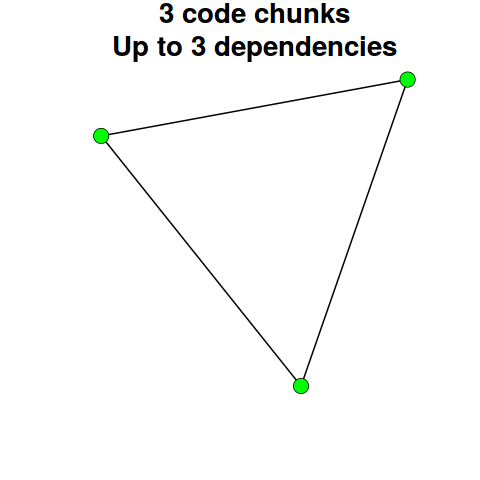
\includegraphics[width=0.31\textwidth]{dependencies3.png}
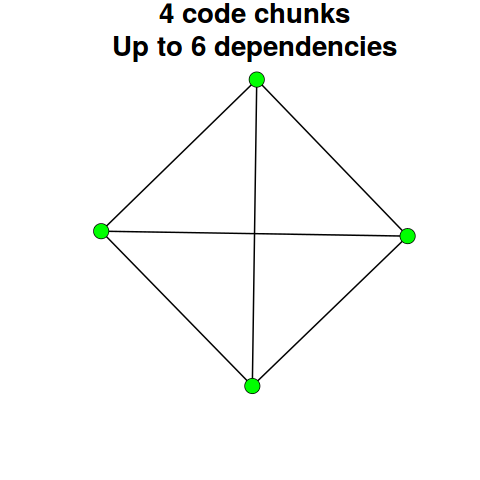
\includegraphics[width=0.31\textwidth]{dependencies4.png}
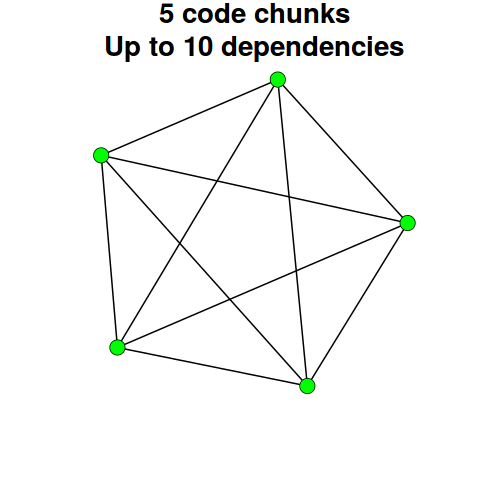
\includegraphics[width=0.31\textwidth]{dependencies5.png}

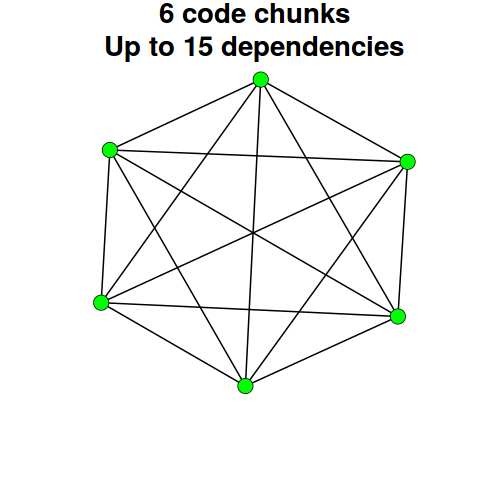
\includegraphics[width=0.31\textwidth]{dependencies6.png}
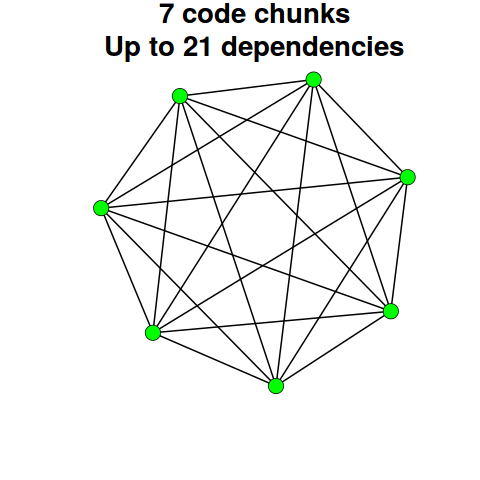
\includegraphics[width=0.31\textwidth]{dependencies7.png}
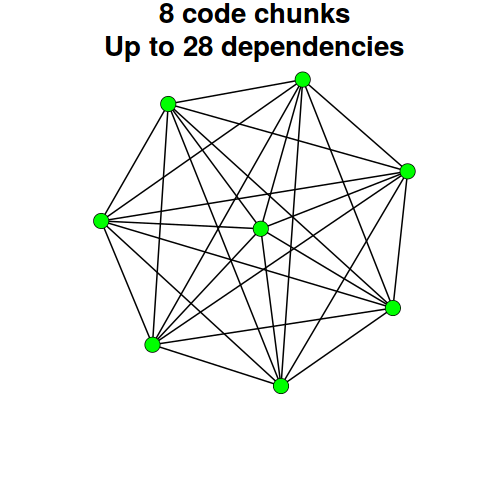
\includegraphics[width=0.31\textwidth]{dependencies8.png}
\caption{The maximum possible number of dependencies for programs of different
sizes.}
\label{fig:dependencyGrowth}
\medskip
\end{figure}

Figure~\ref{fig:dependencyGrowth} quantifies this further, and in fact finally
gives us the insight we need into the cause of the curve in
Figure~\ref{fig:complexityCurve} (on p.~\pageref{fig:complexityCurve}). As you
may remember from Discrete Math class, the number of possible edges in a graph
goes up as the \textit{square} of the number of vertices. (Specifically, a
graph with $n$ vertices can have up to $\frac{n\dot(n-1)}{2}$ edges.) So
doubling the number of code chunks approximately \textit{quadruples} the
number of possible dependencies in the program. That explains why
Figure~\ref{fig:complexityCurve} was \textbf{superlinear} (\textit{i.e.},
increased faster than a straight line would have), and why everyone in the
'70's was underestimating how much time it would take to write and maintain
large programs.

\section{Encapsulation}

\section{Features of OO}

% \section{Exercises}
% 
% Use an index card or a piece of paper folded lengthwise, and cover up the
% right-hand column of the exercises below. Read each exercise in the
% left-hand column, answer it in your mind, then slide the index card down to
% reveal the answer and see if you're right! For every exercise you missed,
% figure out why you missed it before moving on.
% 
% \begin{small}
% \begin{enumerate}
% \newcolumntype{Q}{>{\arraybackslash}m{.3\textwidth}}
% \newcolumntype{A}{>{\arraybackslash}m{.6\textwidth}}
% %\begin{longtable}{m{0.3\textwidth} || m{0.6\textwidth}}
% \begin{longtable}{Q || A}
% \hline
% \item 
% What key software problem was the OO paradigm invented to address?
% &
% Too many dependencies.
% \\
% \hline
% 
% \end{longtable}
% \end{enumerate}
% \end{small}
